68. $y=\cfrac{6|x-3|}{x^2-3x}=\cfrac{6|x-3|}{x(x-3)}=\begin{cases} \cfrac{6}{x},\ x>3,\\ -\cfrac{6}{x},\ x<3.\end{cases}$
$$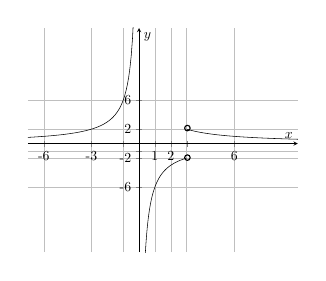
\begin{tikzpicture}[scale=0.5]
\begin{axis}[
    axis lines = middle,
    grid=major,
    legend pos={south west},
    xlabel = {$x$},
    %xlabel style={below right},
    ylabel = {$y$},
    ymin=-15,
    ymax=16,
    xmin=-7,
    xmax=10,
    xtick={-6,-3,-1,1,2,3,6},
    xticklabels={-6,-3,$ $,1,2,$ $,6},
    ytick={-1,-2,-6,2,6},
    yticklabels={$ $,-2,-6,2,6},
                  ]
	\addplot[domain=3:10, samples=100, color=black] {(6/x)};
    \addplot[domain=-8:-0.01, samples=100, color=black] {-(6/x)};
    \addplot[domain=0.01:3, samples=100, color=black] {-(6/x)};
    %\addplot[domain=2.01:6, samples=100, color=black] {2/(2-x)};
   % \addplot[domain=-3:3, samples=100, color=black] {-x};
     %\addlegendentry{$\text{Рис. 1}$};
\end{axis}
\draw (4.05,3.15) circle (2pt);
\draw (4.05,2.4) circle (2pt);
\end{tikzpicture}$$
По графику определим $m\in(-\infty;-2]\cup(2;+\infty).$\\
